\textbf{ \large  Sao dãy chính \href{https://www.wikiwand.com/en/Main_sequence}{(Main sequence stars)}}

Trong bài này, chúng ta hãy cùng xây dựng hệ phương trình cấu trúc của một ngôi sao dãy chính và ước tính các thông số cơ bản của Mặt Trời.

Mặt Trời là một ngôi sao dãy chính(dãy trên hình vẽ dễ thấy nhất từ phía dưới bên phải lên đến phía trên bên trái), với nhiệt độ bề mặt và độ trưng năng lượng được biểu thị trên giản đồ Hertzsprung-Russell.
\begin{figure}[h!]
    \centering
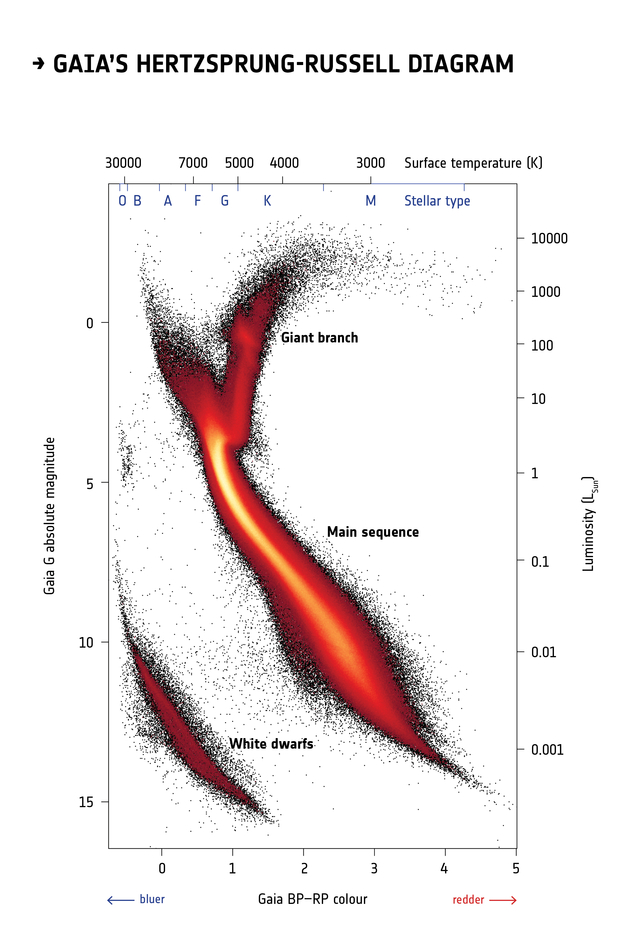
\includegraphics[height=0.65\textheight]{Problem_12/hinh1.jpg}
    \caption{Hình vẽ biểu diễn giản đồ HR của các ngôi sao được đo đạc bởi Gaia, với độ trưng năng lượng $L$ của ngôi sao tỉ lệ với độ trưng năng lượng của mặt trời 1 trên trục tung bên phải, và nhiệt độ bề mặt $T_e(\si{K})$  trên trục hoành ở phía trên.}
\end{figure}
\newpage

\begin{enumerate}
\item Xét lớp cầu khối lượng $dm$ dày $dr$, bán kính $r$, có mật độ khối lượng là $\rho$. Một ngôi sao ở trạng thái cân bằng thuỷ tĩnh khi mà lực hấp dẫn của chính nó cân bằng với nội áp suất từ bên trong ngôi sao tạo ra. Gọi áp suất tác dụng lên mặt trong lớp cầu là $p(r)$, áp suất tác dụng lên mặt ngoài lớp cầu là $p(r+dr)$. Tìm  $\dfrac{dm}{dr}$ và gradient áp suất $\dfrac{dp}{dr}$ để một ngôi sao ở trạng thái cân bằng.
\end{enumerate}
\begin{center}
    

\begin{tikzpicture}[]
    \tkzDefPoint(-3,-3){A}
    \tkzDefPoint(0,-3){D}
    \tkzDrawCircle[fill=battleshipgrey!12,thick](A,D)
    \tkzDrawPoint[color=red,thick](A)
    \tkzDefPoint(-0.8,-3){C}
    \tkzDrawCircle[fill=white,thick](A,C)
    \tkzDefPoint(-1,-3){B}
    \tkzDrawCircle[fill=battleshipgrey!12,thick](A,B)
    
    \tkzDefPointBy[rotation = center A angle 60](B)\tkzGetPoint{D}
    \tkzDrawSegment[thick,->](A,D)
    \tkzDefPointBy[rotation = center A angle 30](C)\tkzGetPoint{E}
    \tkzDrawSegment[thick,->](A,E)
    \tkzLabelSegment[above=1pt](A,D){$r$}
    \tkzLabelSegment[below=1pt,rotate=30](A,E){$r+dr$}
    \tkzDefPoint(0.5,-3){F}
    \tkzDefPoint(-0.8,-3){L}
    \tkzDrawSegment[->](F,L)
    \tkzLabelPoint[right](F){$dm$}
\end{tikzpicture}
\end{center}
Cho phân bố vật chất bên trong mặt trời:

\begin{equation}
\rho(x)=293\exp{(-10.5x)}-139\exp{(-22.7x)} ,
\end{equation}
trong đó $x=\dfrac{r}{R}$.

Áp suất tác dụng lên lớp ngoài cùng của Mặt trời đến từ sự suy giảm bức xạ photon trong quang quyển của mặt trời. Độ dày quang học là một đại lượng đặc trưng cho sự suy giảm đó. Cho biết độ dày quang học của photon là:

\begin{equation}
    \tau(R)=\int_R^\infty \kappa \rho dr =\dfrac{2}{3},
\end{equation}
với $\kappa$ có thể coi là hằng số khi $r>R$. 
\begin{enumerate}[resume]
    \item Tính áp suất $P_\text{s}$ ở bề mặt Mặt Trời, từ đó tính áp suất tại tâm Mặt Trời, biết tâm mặt trời có thể coi là $0.1\%$ bán kính.
\end{enumerate}
\begin{enumerate}[resume]
        \item Thành phần của tâm mặt trời bao gồm 74\% Hidro, 24\% Heli và 2\% các kim loại nặng khác. Tại trung tâm của ngôi sao, do nhiệt đô cao nên vật chất tồn tại ở thể plasma (vật chất bị ion hoá hoàn toàn) nên nó có khối lượng mol khoảng $\mu_i=0.62 \si{g \cdot mol^{-1}}$. Coi khí plasma là khí lý tưởng, ước tính nhiệt độ $T_\text{c}$ ở tâm mặt trời.
\end{enumerate}

Do sự chênh lệch nhiệt độ giữa tâm và bề mặt của một ngôi sao, năng lượng có xu hướng "chảy" từ trong ra ngoài thông qua bức xạ điện từ. Ta hãy xem xét lực do bức xạ tác dụng lên lớp cầu $dm$ trong trường hợp này.
Khi một bức xạ xuyên qua một môi trường truyền thì năng lượng của nó bị chất truyền dẫn đó hấp thụ một phần. Cụ thể, cường độ của bức xạ đó sau khi đi được quãng đường $x$ trong môi trường truyền có mật độ khối lượng $\rho$ và độ mờ $\kappa$ được miêu tả bằng hàm
\begin{equation}
    I(x)=I_0 \exp{(\kappa \rho x)}.
\end{equation}
\begin{enumerate}[resume]
    \item Biết năng lượng bức xạ tới lớp cầu $dr$ trong một đơn vị thời gian là $l(r)$. Tính áp suất bức xạ $dp_{\text{rad}}$ gây ra trên lớp cầu.
    
\end{enumerate}
\begin{enumerate}[resume]
    \item Cho độ mờ trung bình của mặt trời là $\langle \kappa \rangle = 10^2 \si{m^2 \cdot kg^{-1}}$. Độ trưng năng lượng Eddington là độ trưng lớn nhất có thể có của một ngôi sao. Tìm độ trưng Eddington của Mặt Trời.
\end{enumerate}
Người ta tìm thấy rằng áp suất bức xạ bằng một phần ba mật độ năng lượng bức xạ vật đen, kết hợp với định luật Stefan-Boltzmann, ta được: 
\begin{equation}
    p=\dfrac{u}{3}=\dfrac{4\sigma}{3c} T^4 = \dfrac{a}{3}T^4 ,
\end{equation} 

trong đó $a$ được gọi là hằng số bức xạ.
\begin{enumerate}[resume]
    \item Tìm quy luật phân bố nhiệt độ bên trong một ngôi sao dãy chính.   
    \item Cho năng lượng tạo ra do phản ứng hạt nhân của một ngôi sao trong một đơn vị thời gian và trên một đơn vị khối lượng là $\epsilon$. Tìm quy luật phân bố độ trưng năng lượng của một ngôi sao. Độ trưng năng lượng của một ngôi sao tỉ lệ với luỹ thừa bậc mấy của nhiệt độ ? Từ đó so sánh với giản đồ HR và nhận xét. Thời gian một ngôi sao tồn tại ở dãy chính tỉ lệ thế nào với khối lượng của nó.
\end{enumerate}


\begin{enumerate}[resume]
    
    \item Thời khắc cuối cùng của một ngôi sao ở dãy chính diễn ra khi mà Hidro bị chuyển hoá hết thành Heli. Do tốc độ phản ứng tỉ lệ với nhiệt độ, nên khi Hidro ở trong tâm bị sử dụng hết, thì ở phía ngoài, nơi nhiệt độ thấp hơn, Hidro vẫn đang được đốt cháy, tạo ra một lớp vỏ Hidro ở phía ngoài. Khi lõi Heli bên trong đạt tới khối lượng khi mà nó sụp đổ do áp suất của lớp vỏ bên ngoài, gọi là giới hạn Schönberg-Chandrasekhar thì ngôi sao bước vào giai đoạn Sao khổng lồ đỏ. Tìm giới hạn Schönberg-Chandrasekhar $\dfrac{M_\text{c}}{M}$ theo tỉ số $\dfrac{\mu_\text{c}}{\mu_\text{s}}$, với $M_\text{c}$, $M$, $\mu_\text{c}$, $\mu_\text{s}$ lần lượt là khối lượng lõi, khối lượng ngôi sao, khối lượng nguyên tử của lõi và khối lượng nguyên tử của lớp vỏ.  
\end{enumerate}

\begin{flushright}
    (Biên soạn bởi Hiagari)
\end{flushright}